% Options for packages loaded elsewhere
\PassOptionsToPackage{unicode}{hyperref}
\PassOptionsToPackage{hyphens}{url}
%
\documentclass[
]{article}
\usepackage{amsmath,amssymb}
\usepackage{iftex}
\ifPDFTeX
  \usepackage[T1]{fontenc}
  \usepackage[utf8]{inputenc}
  \usepackage{textcomp} % provide euro and other symbols
\else % if luatex or xetex
  \usepackage{unicode-math} % this also loads fontspec
  \defaultfontfeatures{Scale=MatchLowercase}
  \defaultfontfeatures[\rmfamily]{Ligatures=TeX,Scale=1}
\fi
\usepackage{lmodern}
\ifPDFTeX\else
  % xetex/luatex font selection
\fi
% Use upquote if available, for straight quotes in verbatim environments
\IfFileExists{upquote.sty}{\usepackage{upquote}}{}
\IfFileExists{microtype.sty}{% use microtype if available
  \usepackage[]{microtype}
  \UseMicrotypeSet[protrusion]{basicmath} % disable protrusion for tt fonts
}{}
\makeatletter
\@ifundefined{KOMAClassName}{% if non-KOMA class
  \IfFileExists{parskip.sty}{%
    \usepackage{parskip}
  }{% else
    \setlength{\parindent}{0pt}
    \setlength{\parskip}{6pt plus 2pt minus 1pt}}
}{% if KOMA class
  \KOMAoptions{parskip=half}}
\makeatother
\usepackage{xcolor}
\usepackage[margin=1in]{geometry}
\usepackage{longtable,booktabs,array}
\usepackage{calc} % for calculating minipage widths
% Correct order of tables after \paragraph or \subparagraph
\usepackage{etoolbox}
\makeatletter
\patchcmd\longtable{\par}{\if@noskipsec\mbox{}\fi\par}{}{}
\makeatother
% Allow footnotes in longtable head/foot
\IfFileExists{footnotehyper.sty}{\usepackage{footnotehyper}}{\usepackage{footnote}}
\makesavenoteenv{longtable}
\usepackage{graphicx}
\makeatletter
\def\maxwidth{\ifdim\Gin@nat@width>\linewidth\linewidth\else\Gin@nat@width\fi}
\def\maxheight{\ifdim\Gin@nat@height>\textheight\textheight\else\Gin@nat@height\fi}
\makeatother
% Scale images if necessary, so that they will not overflow the page
% margins by default, and it is still possible to overwrite the defaults
% using explicit options in \includegraphics[width, height, ...]{}
\setkeys{Gin}{width=\maxwidth,height=\maxheight,keepaspectratio}
% Set default figure placement to htbp
\makeatletter
\def\fps@figure{htbp}
\makeatother
\setlength{\emergencystretch}{3em} % prevent overfull lines
\providecommand{\tightlist}{%
  \setlength{\itemsep}{0pt}\setlength{\parskip}{0pt}}
\setcounter{secnumdepth}{5}
\newlength{\cslhangindent}
\setlength{\cslhangindent}{1.5em}
\newlength{\csllabelwidth}
\setlength{\csllabelwidth}{3em}
\newlength{\cslentryspacingunit} % times entry-spacing
\setlength{\cslentryspacingunit}{\parskip}
\newenvironment{CSLReferences}[2] % #1 hanging-ident, #2 entry spacing
 {% don't indent paragraphs
  \setlength{\parindent}{0pt}
  % turn on hanging indent if param 1 is 1
  \ifodd #1
  \let\oldpar\par
  \def\par{\hangindent=\cslhangindent\oldpar}
  \fi
  % set entry spacing
  \setlength{\parskip}{#2\cslentryspacingunit}
 }%
 {}
\usepackage{calc}
\newcommand{\CSLBlock}[1]{#1\hfill\break}
\newcommand{\CSLLeftMargin}[1]{\parbox[t]{\csllabelwidth}{#1}}
\newcommand{\CSLRightInline}[1]{\parbox[t]{\linewidth - \csllabelwidth}{#1}\break}
\newcommand{\CSLIndent}[1]{\hspace{\cslhangindent}#1}
\ifLuaTeX
  \usepackage{selnolig}  % disable illegal ligatures
\fi
\IfFileExists{bookmark.sty}{\usepackage{bookmark}}{\usepackage{hyperref}}
\IfFileExists{xurl.sty}{\usepackage{xurl}}{} % add URL line breaks if available
\urlstyle{same}
\hypersetup{
  pdftitle={Lessons learned: creating tutorials teaching Agent-Based Modelling for Archaeologists},
  hidelinks,
  pdfcreator={LaTeX via pandoc}}

\title{Lessons learned: creating tutorials teaching Agent-Based Modelling for Archaeologists}
\author{true \and true \and true \and true \and true \and true \and true \and true \and true}
\date{05 March 2024}

\begin{document}
\maketitle

{
\setcounter{tocdepth}{2}
\tableofcontents
}
\hypertarget{introduction}{%
\section{Introduction}\label{introduction}}

ABM application increased in Archaeology

Other teaching material available SPOC (Scherjon, Romanowska and Lambers 2019)

New handbook (Romanowska, Wren and Crabtree 2021)

No formal training

EU project \url{https://erasmus-plus.ec.europa.eu/nl/projects/search/details/2021-2-IE01-KA220-VET-000049054}

\hypertarget{method}{%
\section{Method}\label{method}}

During the project we have developed tutorials. The tutorials were first designed using storyboards which were later converted into tutorials using NetLOGO Web (\url{https://www.netlogoweb.org/launch}) and Javascript (). The tutorials were developed together and we worked together using GitHub (\url{https://github.com/lljvdk/EU-ABMA/}). During the project initial testing was done with all authors and issues in GitHub were used to tackle bugs.

The learning and teaching material for ABM for archaeologists assumes that the users have completed secondary education. It is suitable for archaeologists with at least some background in archaeology and preferably after at least the first year of a Bachelor study in Archaeology (preferably above EQF levels 4 or 5). In addition, the tutorials are aimed at professionals working in archaeology and some experience with computer. We also assume that learners are proficient in English and have at least the Reading B1 level, but Reading B2 is recommended (Council of Europe 2020). The tutorials are developed aiming to develop learners in the following competence area's: 1. Information and data literacy, 2. Communication and collaboration, 3. Digital content creation and, 5. Problem solving (European Commission, Joint Research Centre et al. 2022).

The tutorial were tested during various online and in-person conferences. The in-person conferences were attended by several people from the project team. During the online events we were always present with several people and enabled participants to go to break-out rooms if they needed any help or wanted to discuss things. In addition, we also had students working with the tutorials at Saxion University of applied sciences and Leiden University. We used the feedback of the participants to improve the tutorials. The feedback was obtained structurally using two surveys using Qualtrics. The participants of the events were asked to answer questions of a survey before participating. We used the answers to understand what the background of the participants was and to get an estimate of their level of knowledge in relation to ABM (see appendix \ldots{} for the questions). After the participants worked with the tutorials during the event they were asked to answer a second survey. Questions of this survey were aimed at the measuring the effectiveness of the tutorials and getting feedback on the workshop and tutorials (see appendix \ldots{} for the questions). For some events participants had to register beforehand and we were able to send the pre-workshop survey by email. At other events no registration was possible or necessary and the pre-workshop survey was given at the start of the event. The post-workshop survey was distributed using QR-codes or links at the end of the workshop during the event. After each event we have improved the tutorials based on the received feedback.

\begin{longtable}[]{@{}
  >{\raggedright\arraybackslash}p{(\columnwidth - 8\tabcolsep) * \real{0.2000}}
  >{\raggedright\arraybackslash}p{(\columnwidth - 8\tabcolsep) * \real{0.2000}}
  >{\raggedright\arraybackslash}p{(\columnwidth - 8\tabcolsep) * \real{0.2000}}
  >{\raggedright\arraybackslash}p{(\columnwidth - 8\tabcolsep) * \real{0.2000}}
  >{\raggedright\arraybackslash}p{(\columnwidth - 8\tabcolsep) * \real{0.2000}}@{}}
\caption{Conferences, events and situations were the workshops given and the tutorials were tested.}\tabularnewline
\toprule\noalign{}
\begin{minipage}[b]{\linewidth}\raggedright
Conference or event
\end{minipage} & \begin{minipage}[b]{\linewidth}\raggedright
Period
\end{minipage} & \begin{minipage}[b]{\linewidth}\raggedright
Online, in person or hybrid
\end{minipage} & \begin{minipage}[b]{\linewidth}\raggedright
Number of participants
\end{minipage} & \begin{minipage}[b]{\linewidth}\raggedright
Number of registrations
\end{minipage} \\
\midrule\noalign{}
\endfirsthead
\toprule\noalign{}
\begin{minipage}[b]{\linewidth}\raggedright
Conference or event
\end{minipage} & \begin{minipage}[b]{\linewidth}\raggedright
Period
\end{minipage} & \begin{minipage}[b]{\linewidth}\raggedright
Online, in person or hybrid
\end{minipage} & \begin{minipage}[b]{\linewidth}\raggedright
Number of participants
\end{minipage} & \begin{minipage}[b]{\linewidth}\raggedright
Number of registrations
\end{minipage} \\
\midrule\noalign{}
\endhead
\bottomrule\noalign{}
\endlastfoot
CAA Amsterdam & April 2023 & In person & 36 & 53 \\
EAA Belfast & August 2023 & In person & 21 & No registration \\
CAA-DE/NL-Fl Online workshop & October 2023 & Online & 40 & 76 \\
Reuvensdagen & November 2023 & In person & 13 & No registration \\
CAA-UK & November 2023 & Hybrid & 53 & \\
Leiden (course) & December 2023 & In person & 11 & No registration \\
Aarhus & January/February 2024 & Online & 176 & \textgreater500 \\
Saxion & March 2023-January 2024 & In person & 18 & No registration \\
\textbf{Total} & & & \textbf{368} & \textbf{\textgreater628} \\
\end{longtable}

The surveys were analysed using R (R Core Team 2023). The following packages were used for analyses: ggplot2 (Wickham 2016), dplyr (Wickham et al. 2023), tidyr (Wickham, Vaughan and Girlich 2023), forcats(Wickham 2023a), lubridate (Grolemund and Wickham 2011) and stringr (Wickham 2023b). The date and the code is available at \url{https://github.com/RonaldVisser/ABM_tutorials} and (\ldots{} insert Zenodo reference\ldots)

Over the course of the project three groups of students worked on the project during the Smart Solutions Semester at Saxion University of Applied Sciences. This is an interdisciplinary semester in which students of at least three different study-programmes or disciplines work together on a complex problem/project (\url{https://www.saxion.edu/business-and-research/collaborate-with-saxion/smart-solutions}). The backgrounds of the various students were diverse: Applied Computer Science, Archaeology, Business Management Studies, Creative Business, Creative Media \& Game Technologies, and ICT. The diverse groups of students contributed with new ideas, developing educational material, testing the tutorials and developing a style for the website and other materials.

\hypertarget{results}{%
\section{Results}\label{results}}

\hypertarget{workhops-and-tutorials}{%
\subsection{Workhops and tutorials}\label{workhops-and-tutorials}}

\hypertarget{final-tutorials}{%
\subsection{Final tutorials}\label{final-tutorials}}

The set of developed tutorials consists of the following tutorials:

\begin{itemize}
\item
  Tutorial 1: Introduction to ABM
\item
  Tutorial 2: Beginning with NetLogo
\item
  Tutorial 3: Expanded ABM skills
\item
  Tutorial 4: Intermediate ABM
\item
  Tutorial 5: How to Model
\end{itemize}

Each tutorials consists of a different number of lessons that guide the learner in a self-pace manner through the lessons.

In the first tutorial the learner will learn what simulations and agent-based models are and how they can help in archaeological research. This tutorial consists of 4 lessons. The first two lesson introduce the learner into simulation in general and Agent-Based Modelling in specific. Various concepts related to ABM are introduced and the first concepts within NetLogo are explained. The third lesson aims to explain how ABMs are used in archaeological research. The final lesson introduces the learner to the NetLogo Interface and the difference between the Interactive and Authoring mode. This tutorial build a foundation for working in NetLogo and with ABM. All activity stays within the intermediate level, although higher levels might be touch upon.

In tutorial 2 the learner will learn the basics of NetLogo by making your first simulation on the Out of Africal dispersal of homo sapiens. The leaerner will work with basic NetLogo syntax and learn how to set up a simulation and visualize their outcomes. This tutorial consists of 9 lessons. This tutorial intends to guide the learner from the intermediate to the advanced level of proficiency. The learning curve is relatively gentle. This is achieved by learning to work with the NetLogo web interface. The primitives are introduced and initialization phase of a simple ABM is gone through. The world within NetLogo's world (including dimensions, coordinates, origin) and how to alter it are explained and experience in a hands-on approach. The learners learn about simple simulation loops and how to use primitives. The advanced level is achieved with the custom procedures and variables. In addition, if-statements are introduced and more complex versions thereof. Exporting information using plots is also explained.

In the third tutorial, the learner will build a simple trade model, picking up more advanced NetLogo coding along the way, such as loops, lists and reporters. The learner will be introduced to some techniques like modular code development and debugging which will become important with this increased coding complexity. This tutorial consists of 7 lessons. This tutorial intends to guide the learner from the intermediate to the advanced and highly specialised level of proficiency. This is achieved by improving development through using modular code, pseudocode and annotating the code. In addition, custom agent breeds are introduced. Visualization with labels and reporters, plots and monitors are learned. The use of loops is further explained. Debugging is learned in lesson 7. This can be very advanced, since it involves knowledge of the NetLogo-language combined with problem solving of unexpected behaviour.

In tutorial 4 the learner will work with Sugarscape simulations to further expand your ABM and NetLogo skills. The learner will learn how to set up more complex interactions between agents and the environment. Furthermore, the basics of setting up good experiments and validating models will be explained. This tutorial consists of 8 lessons. This tutorial intends to guide the learner from the (intermediate and) advanced level to the highly specialised level of proficiency. In this tutorial more complex agent-environment interaction is further learned, including learning ways to visualize the environment and how to give more agency to patches. Creating toy landscapes are central to lesson 5. The learner also learns the basics of setting up experiments in NetLogo and how to use monitors and flexible plots to understand the results. The validation of agent-based models is an important concept of designing a good experiment. The finale step, is to compare simulation results with the archaeological record. The last lesson is aimed at learning syntax to make lists more dynamic and how to refactor code.

In the final and fifth tutorial the learner will learn more about how to actually incorporate agent-based modelling in research. This tutorial focusses less on programming in NetLogo and more on the model development process. The learner will learn about the different phases in modelling and how to export data from models. This tutorial consists of 5 lessons. This tutorial touches upon various levels, but mainly between the intermediate and highly specialised level of proficiency. This tutorial is approaches more theoretical aspects in a practical environment. The learner leans about the model development process starting with the conceptual phase of the model development. Good and bad research questions for modelling are explained and the difference between them. The learner needs to understand how to pick the right modelling technique. The learner should understand the importance of properly conceptualizing a model before starting the technical phase of the model development. In this phase parametrisation, designing experiments and the analyses and interpretation of the models are important. Learning about the dissemination phase of the model development is aimed at understanding (the importance of) publishing models and replication. In addition, learning how to export results from NetLogo using basic export primitives is explained. The BehaviorSpace is explained to enable the learners to analyse the output of models.

\hypertarget{before-the-workshops}{%
\subsection{Before the workshops}\label{before-the-workshops}}

A large proportion of the participants of the workshops gave us information using the survey before the workshops (172 of 368 participants). The respondents came from many different countries all over the world (see Figure \ref{fig:nationality}. The number of female respondents slightly outnumber the male ones and a small group did not share their gender and two were non-binary (see Figure \ref{fig:gender-age}). The ages of the respondents ranged from below 20 to over 70, reaching people in different age classes, although the majority was aged between 20 and 40. It seems that the different events also had a slightly different distribution of both gender and age. For example, more older people attended the workshop at the CAA conference in April 2023 and more male people were present during the workshop at the Reuvensdagen in November 2023.

\begin{figure}
\centering
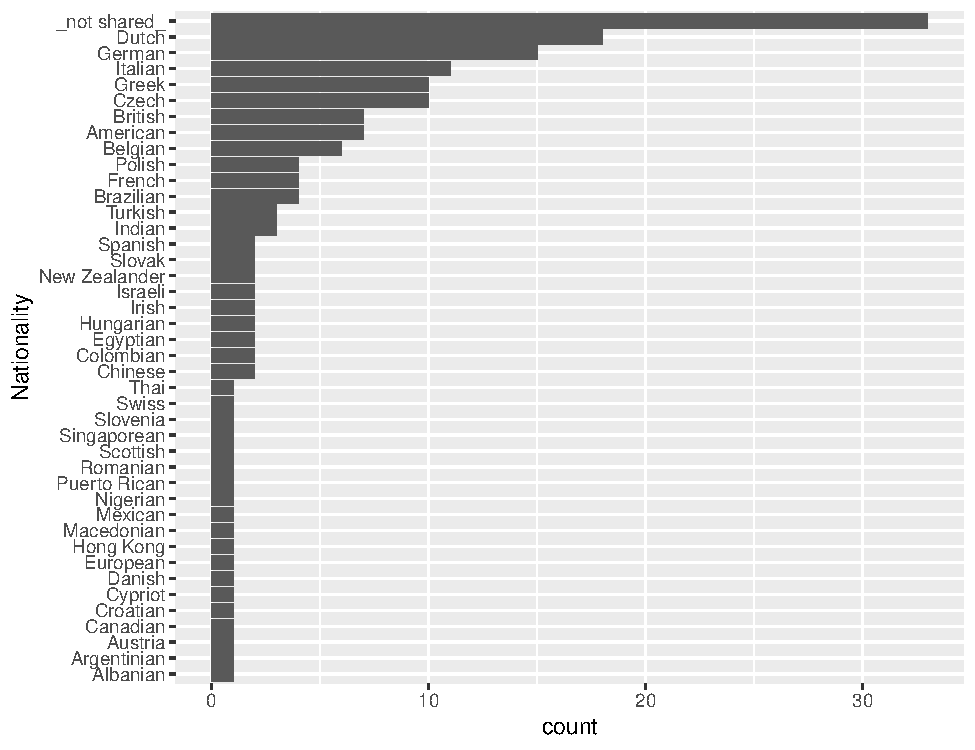
\includegraphics{paper_files/figure-latex/nationality-1.pdf}
\caption{\label{fig:nationality}The nationality of the participants that filled in the survey.}
\end{figure}

\begin{figure}
\centering
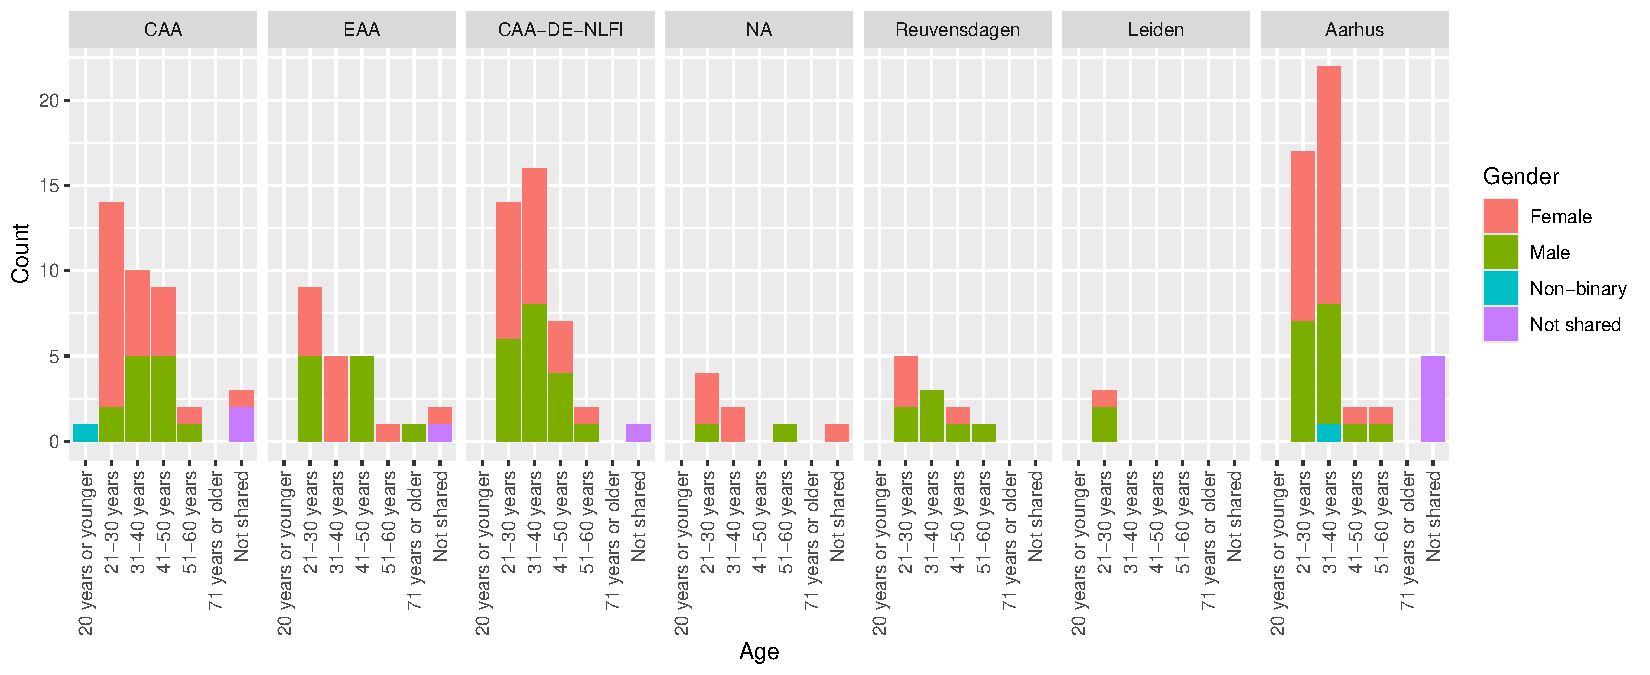
\includegraphics{paper_files/figure-latex/gender-age-1.pdf}
\caption{\label{fig:gender-age}The gender and age of the respondents for each workshop}
\end{figure}

Most of the respondents had several skills with computer applications in archaeology (see Figure \ref{fig:computer-skills}), and many of them did have some knowledge of ABM, although a large group was completely new to the subject. The majority had never applied ABM before participating in the workshops with 14 having applied ABM. It is interesting to note that many respondents did know what kind of software was available for ABM (see Figure \ref{fig:abm-knowledge}).

\begin{figure}
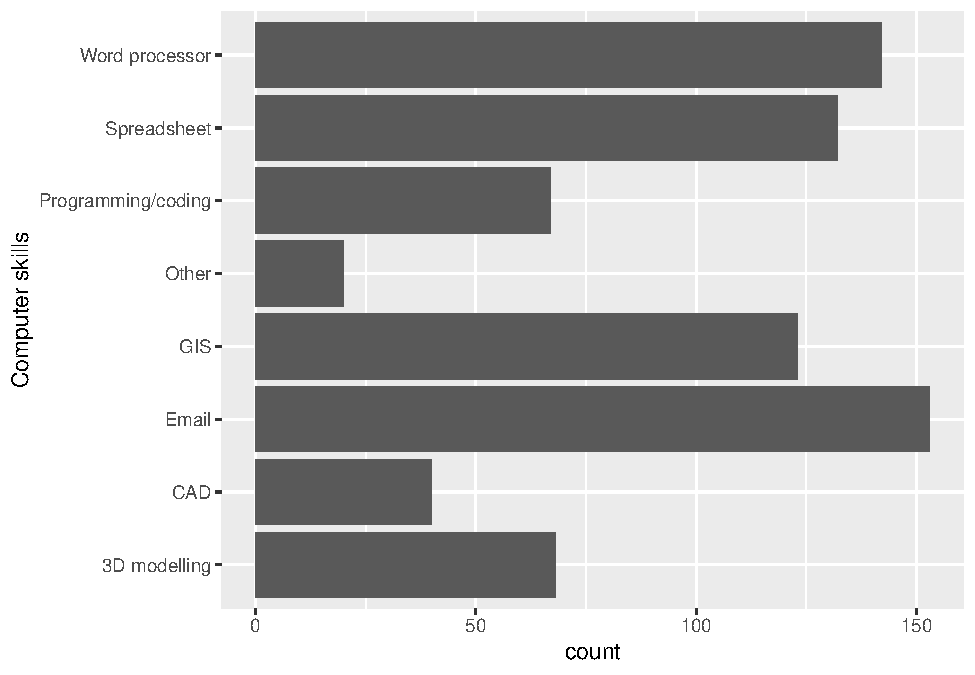
\includegraphics[width=0.5\linewidth]{paper_files/figure-latex/computer-skills-1} \caption{The computer skills of the respondents.}\label{fig:computer-skills}
\end{figure}

\begin{figure}
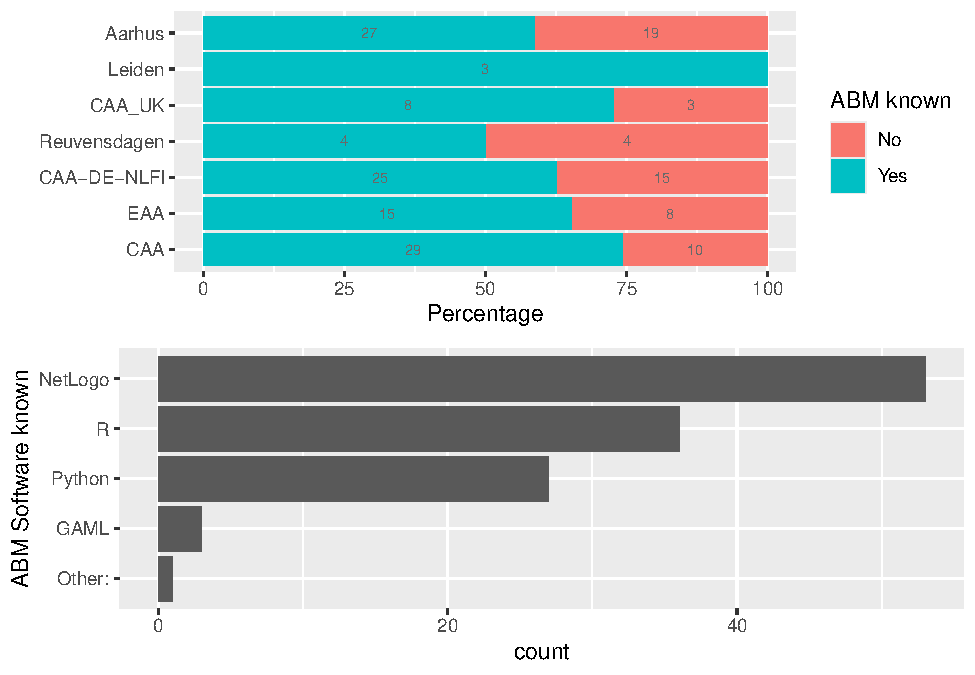
\includegraphics[width=0.5\linewidth]{paper_files/figure-latex/abm-knowledge-1} 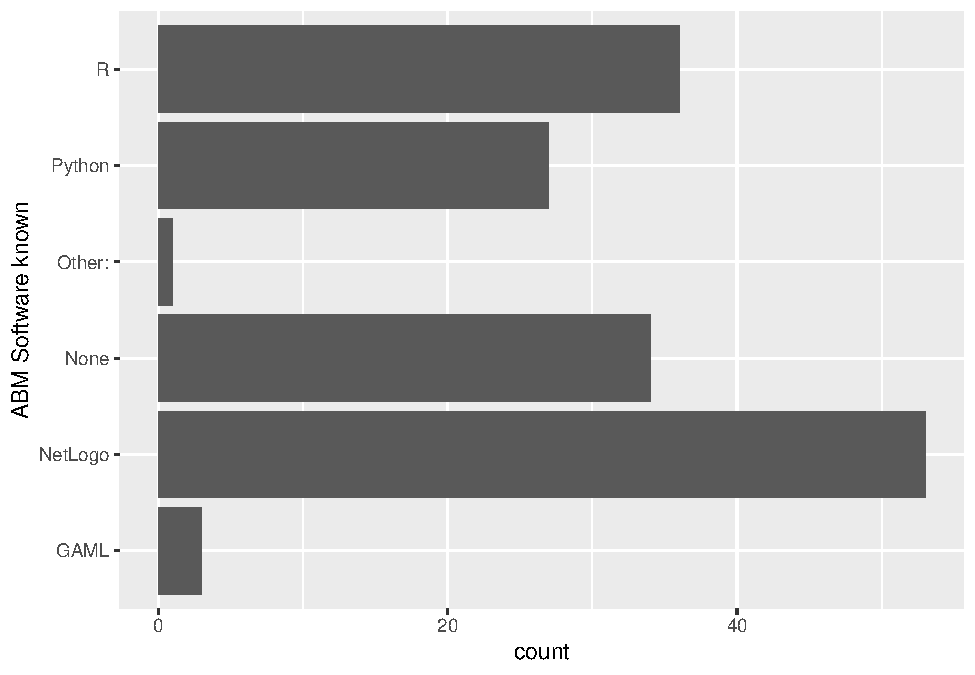
\includegraphics[width=0.5\linewidth]{paper_files/figure-latex/abm-knowledge-2} \caption{Respondents knowledge and experience with ABM.}\label{fig:abm-knowledge}
\end{figure}

As shown above, the respondents had some knowledge on ABM in general, but did not know how to apply this or had never applied this before. The respondents were also asked how they rated the available knowledge on ABM (Figure \ref{fig:available-theory}). While the largest group of them had no opinion on the subject, a very large proportion of the responded answered that they rated the available theory on ABM as limited and a smaller group as sufficient. A minority rated the available theory on ABM as more than sufficient. This clearly shows the need for better educational material.

\begin{figure}
\centering
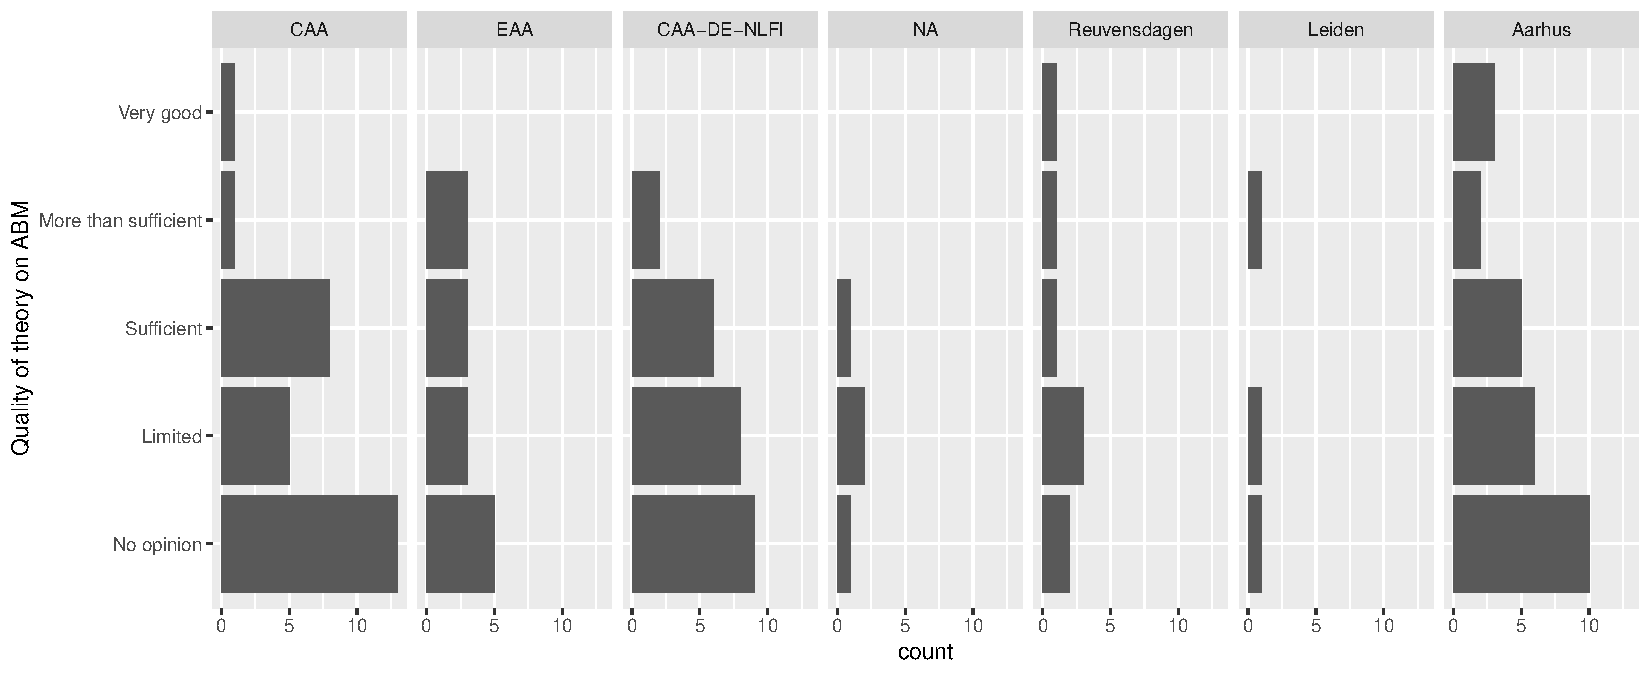
\includegraphics{paper_files/figure-latex/available-theory-1.pdf}
\caption{\label{fig:available-theory}Respondents optionion on the quality of theory on ABM faceted out by event.}
\end{figure}

\hypertarget{during-the-workshop}{%
\subsection{During the workshop}\label{during-the-workshop}}

During the workshops the participants worked in a self-paced manner, often on their own, but sometimes working together and discussing the tutorials. Some particpants engaged in discussion with the teachers to learn how they could apply ABM in their research of discuss possibilities for the application of ABM in general.

\hypertarget{after-workshop}{%
\subsection{After workshop}\label{after-workshop}}

A large proportion of the participants of the workshops gave us information using the survey after the workshops (171 of 368 participants), a similar proportion as those responding to the survey before the workshop.

\begin{figure}
\centering
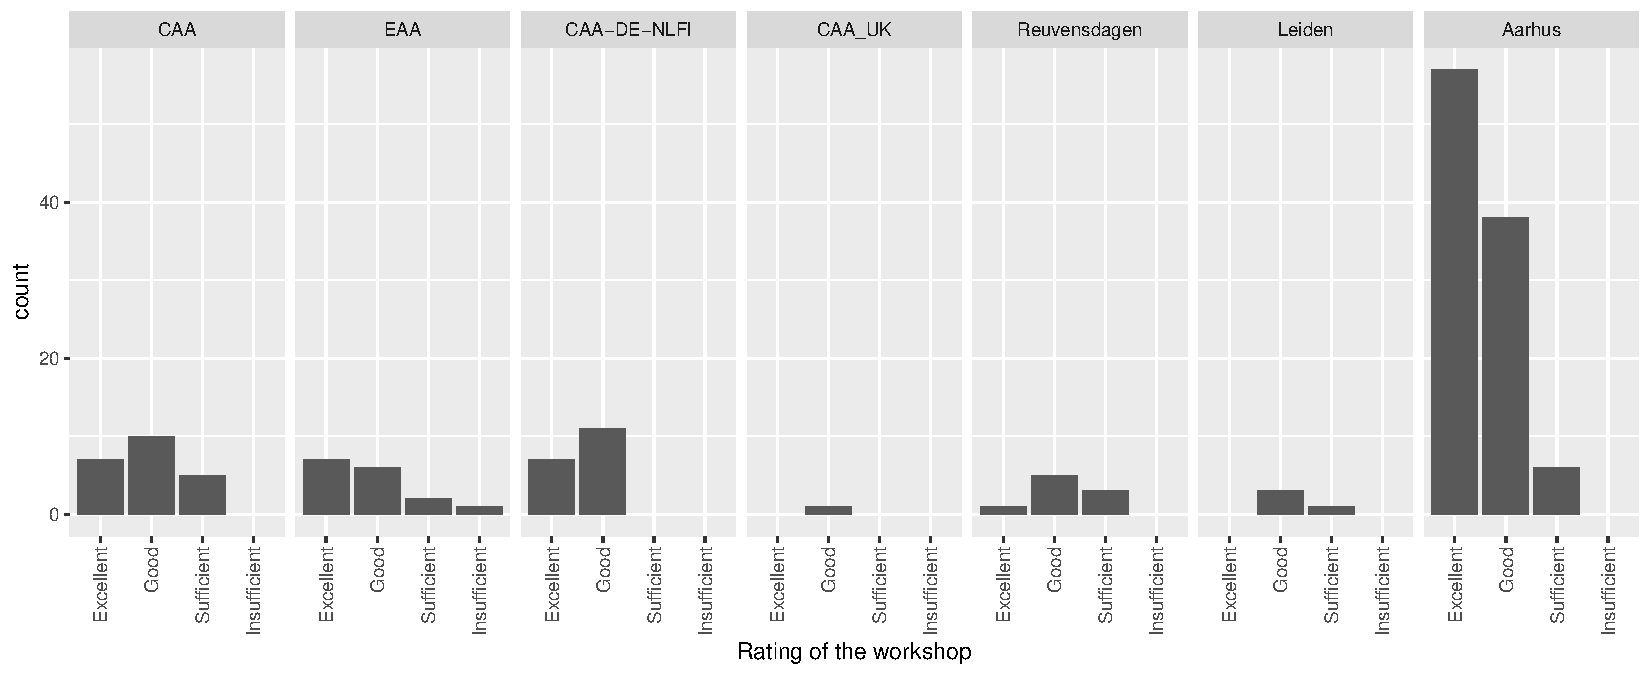
\includegraphics{paper_files/figure-latex/rating-workshop-1.pdf}
\caption{\label{fig:rating-workshop}Respondents rating of the workshop in general faceted for each event.}
\end{figure}

The majority of the respondents were enthusiastic about the teaching material, with the majority rating it as excellent or good. The teachers were even rated better than the teaching material, with more respondents rating them as excellent (see Figure \ref{fig:rating-teaching}).

\begin{figure}
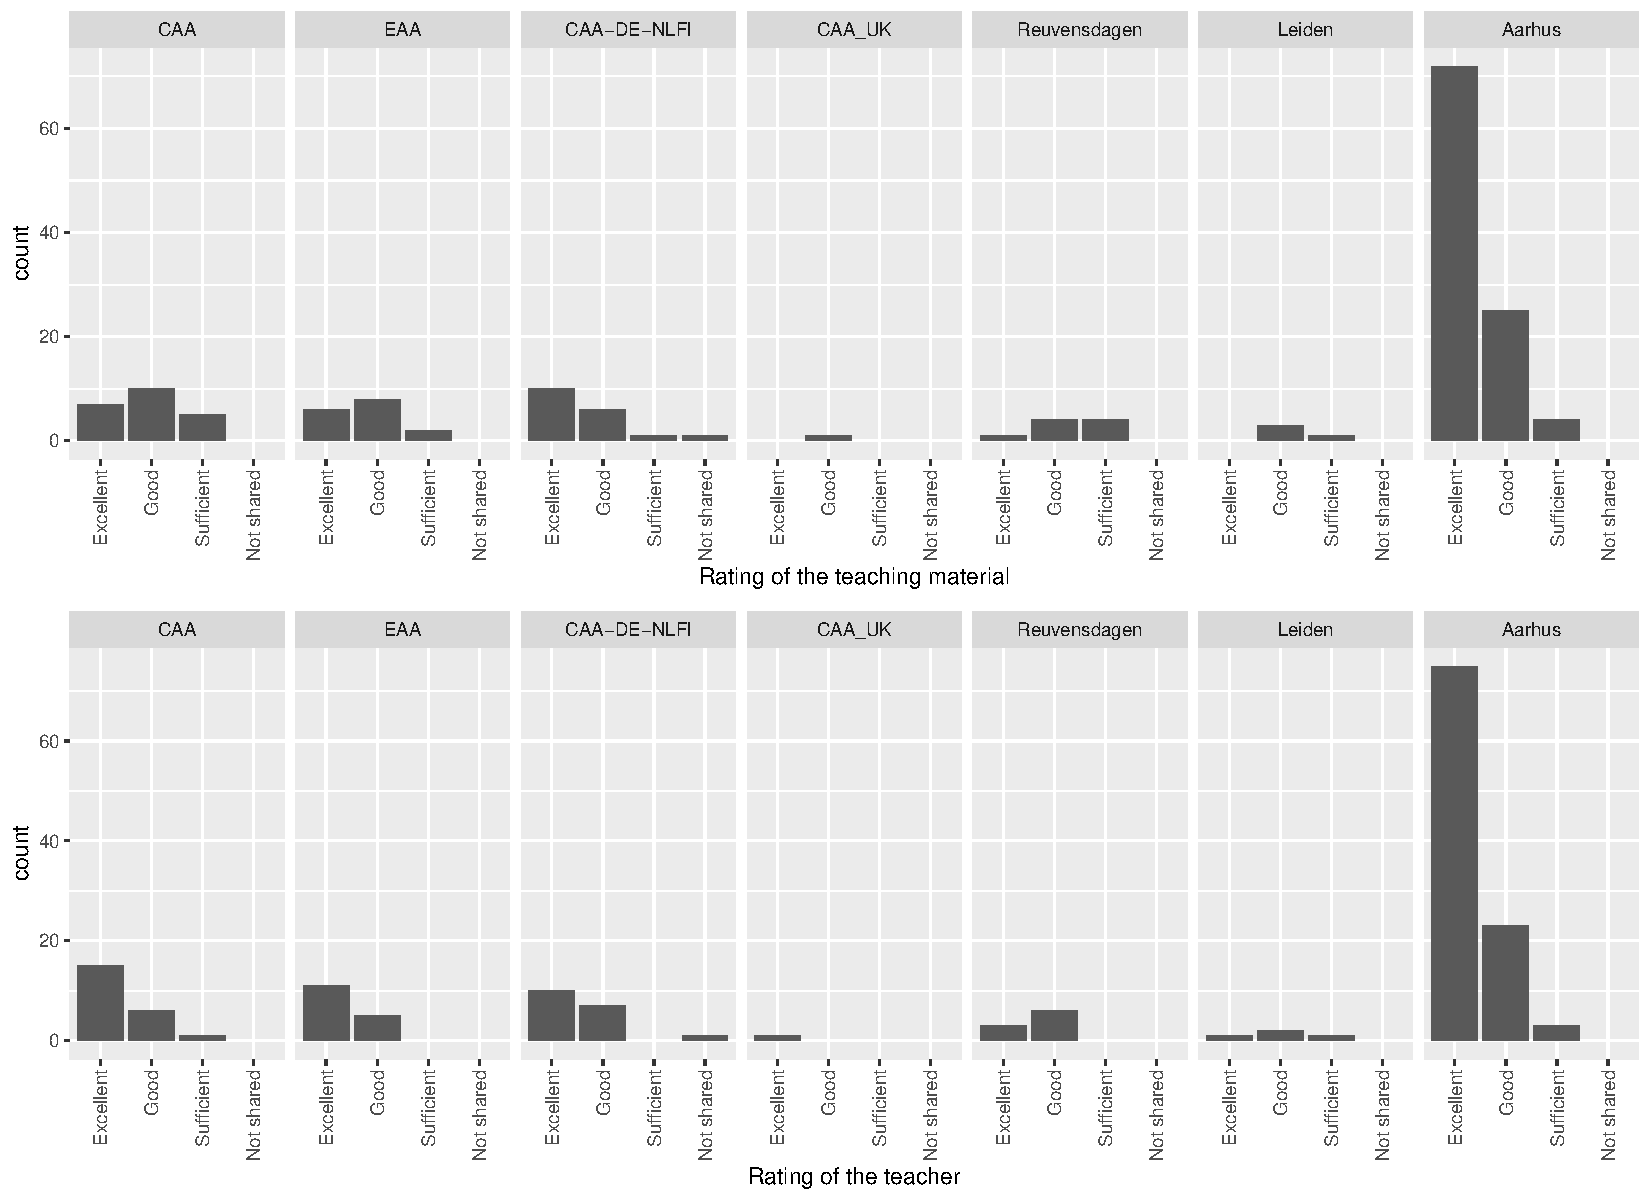
\includegraphics[height=0.5\textheight]{paper_files/figure-latex/rating-teaching-1} 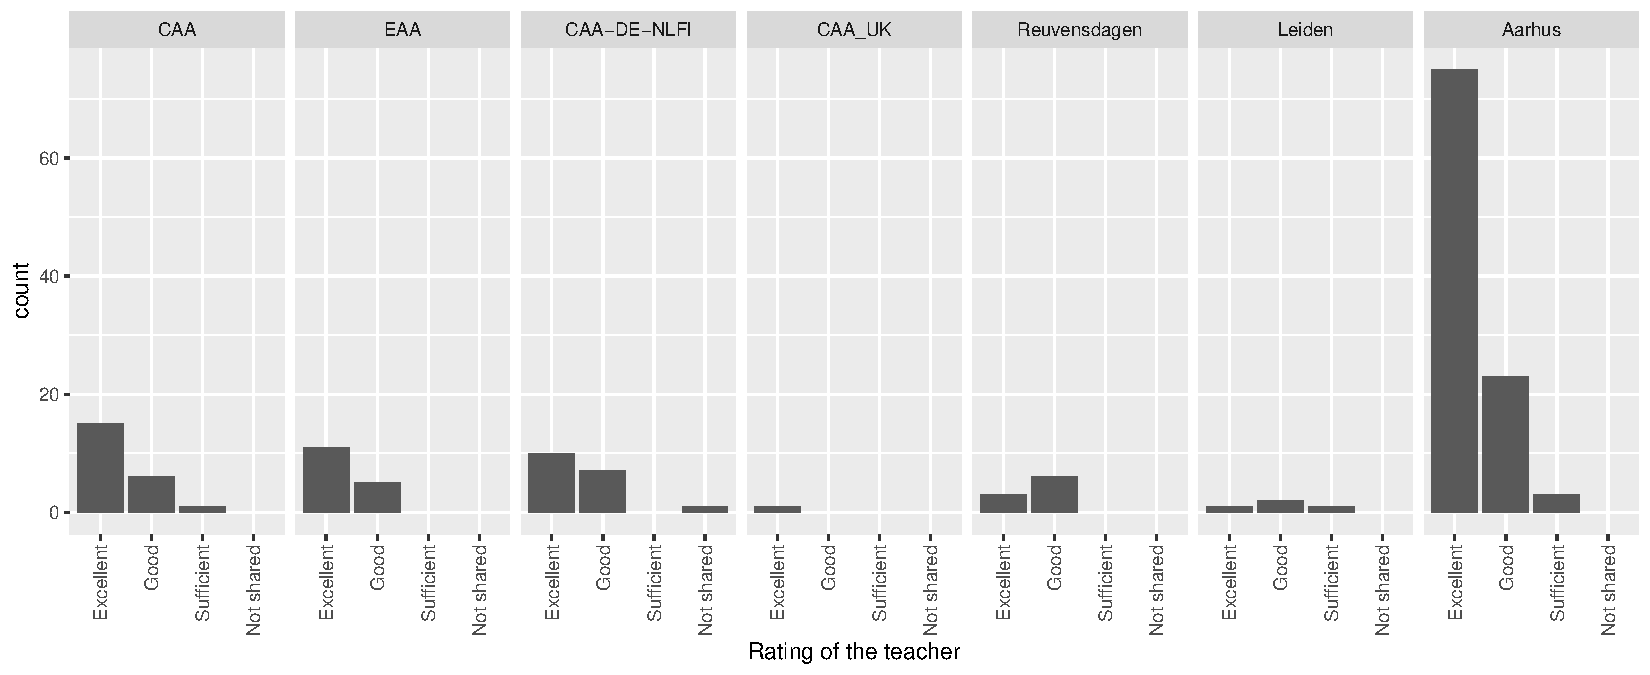
\includegraphics[height=0.5\textheight]{paper_files/figure-latex/rating-teaching-2} \caption{Respondents rating of the teaching material in general faceted for each event.}\label{fig:rating-teaching}
\end{figure}

Two more open questions were asked to the respondents. The first was aimed at getting positive feedback and the other was aimed at getting feedback to improve the tutorials.

The respondents generally liked the interactive step-by-step way of going through the tutorials, but also valued the interaction with the teachers very much. The easy and intuitive introduction into ABM and NetLOGO were also mentioned quite often. This was also observed during the workshops by us, most participants were working in the own pace and did not need much help. From a didactic point of view, the self-paced going through the tutorials is very efficient for teachers.

We also received feedback on possible improvements. For the first workshops we mostly received feedback on the number of bugs. During the CAA-conference in Amsterdam we did the first test of the tutorials and we also instructed the participants that this was work in progress. The number of references to bugs reduced to zero by the end and people started providing other feedback, for example the wish to see more examples or expanding the tutorials more. Some wanted more cooperation, which is possible, but for some online events harder, although we provided break-out rooms. It is also interesting to note that more and more people did not see any room for improvement.

The majority of the respondents that wanted to apply ABM in the future for research (144 of the 164 that answered this question, see Figure \ref{fig:future-abm}). Some of the respondents were already using ABM. A large group was not sure yet in how to apply ABM and wanted to read more on the subject or play a bit with the possibilities. Many respondents also shared the context in which they were thinking to apply ABM to. Various were thinking about movement of people or goods over land or water, sometimes in relation to trade or other distribution mechanisms. Others thought of demography, social networks, migration or settlement distributions patterns. The natural environment and the interaction with humans in the past was also mentioned by some, and often in relation to GIS or how to replace GIS with ABM. The archaeological periods that the participants were interested in were very diverse ranging from the paleolithic to the medieval period.

\begin{figure}
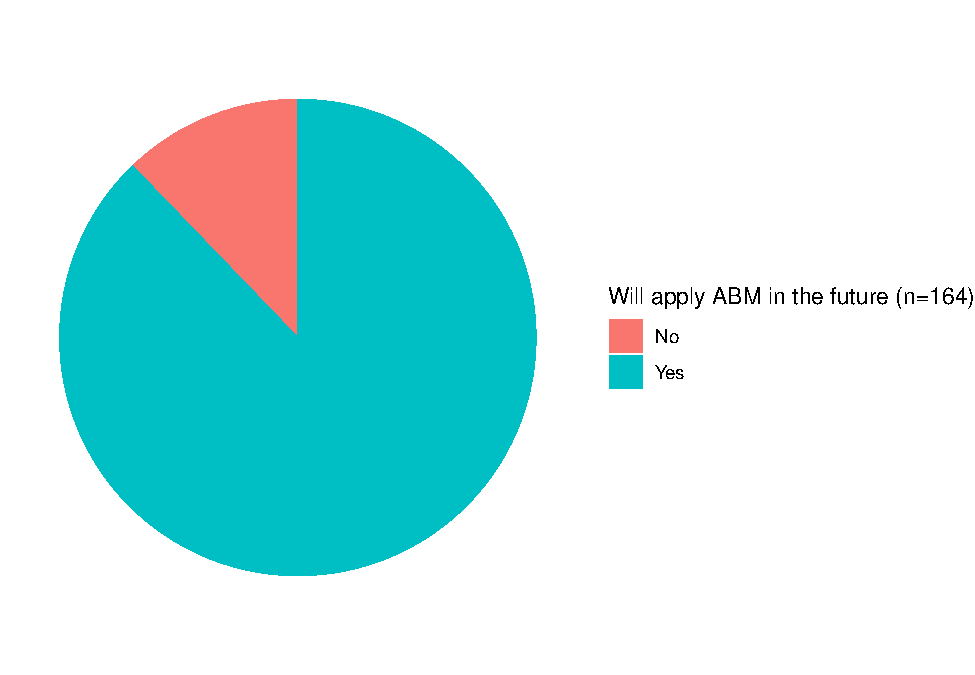
\includegraphics[height=0.5\textheight]{paper_files/figure-latex/future-abm-1} \caption{The respondents reaction to the question if they thing that they will apply ABM in the future.}\label{fig:future-abm}
\end{figure}

\hypertarget{the-digital-competence-framework-for-citizens-2.2}{%
\subsection{The Digital Competence Framework for Citizens (2.2)}\label{the-digital-competence-framework-for-citizens-2.2}}

The tutorials are aimed at developing learners in the following competence area's: 1. Information and data literacy, 2. Communication and collaboration, 3. Digital content creation and, 5. Problem solving (European Commission, Joint Research Centre et al. 2022). In these competence area's various competences are developed towards an advanced or even specialised level.

For competence area 1. Information and data literacy: the tutorials mainly address 1.2 Evaluating Data, Information And Digital Content and 1.3 Managing Data, Information And Digital Content. The users learn about working with data, being critacal of their digital content and how to model and manage the data in the context of an ABM. For tutorial 2 the user is expected to be able to lookup information using the NetLogo(Web) dictionary (\url{http://ccl.northwestern.edu/netlogo/bind/} or \url{http://ccl.northwestern.edu/netlogo/docs/dictionary.html}).

For Competence Area 2. Communication and collaboration the tutorials mainly address 2.1 Interacting Through Digital Technologies, because the users are constantly interacting with digital technologies, but communications is not relevant for the tutorials. However, during the workshops given in the course of the project, participants interacted with each other and the teachers.

Competence Area 3. Digital content creation is one of the main competence area's for the ABM-teaching material. In the process of learning ABM the users are constantly 3.1 Developing Digital Content and 3.2 Integrating And Re-Elaborating Digital Content. The material does not touch upon 3.3 Copyright And Licences, but we assume that users have a general understanding. A very important aspect of learning ABM is 3.4 Programming. The users are exploring the possibilities and chances of programming an ABM. The users are expected to learn both syntax and more general concepts such as modular code development, loops, lists and commenting and documenting code.

Competence Area 5. Problem solving is very important and is closely tied to 3.4 Programming, since programming involves a lot of problem solving. In addition, the creation of a highly complex ABM consists of problem solving all the time, including debugging. All competencies are addressed: 5.1 Solving Technical Problems, is common when writing code, learning about coding, error handling and going from pseudocode to real code. The competence 5.2 Identifying Needs And Technological Responses, is a central issue of the course, while 5.3 Creatively Using Digital Technology is an important aspect of learning to think in models and develop models themselves. In tutorial 2 various aspects of 5.4 Identifying Digital Competence Gaps, are relevant, since this tutorial will force the user to remember code and commands and forces the user to assess their knowledge and skills.

\hypertarget{digital-skills-passport}{%
\subsection{Digital Skills Passport}\label{digital-skills-passport}}

\hypertarget{dissemination-of-tutorials}{%
\subsection{Dissemination of tutorials}\label{dissemination-of-tutorials}}

Website

Github

\hypertarget{conclusion}{%
\section{Conclusion}\label{conclusion}}

Lessons learned

Future aspects

\hypertarget{acknowledgements}{%
\section{Acknowledgements}\label{acknowledgements}}

This project was funded as an Erasmus+ project (\url{https://erasmus-plus.ec.europa.eu/nl/projects/search/details/2021-2-IE01-KA220-VET-000049054}) and we thank the Erasmus+ program for enabling us to make these tutorials.

We would like to thank the student groups at Saxion University of Applied Sciences that worked with us:

\begin{itemize}
\item
  September 2022-February 2023: Dany Dragoi, Liam van den Bosch, Marko Stojkovic, Max van Duinen, Nora van den Engel, Roan Man, Stefan Oostingh and their tutor: Mark Spanjer.
\item
  February 2022-July 2023: Alice Overgaauw, Johan Broersma, Mandy Hazenberg, Paulina Fulneczek, Ties Heesink and their tutor: Jan Willem Huson.
\item
  September 2023-February 2024: Arnfinn Sijbrant, Eva Baan, Jip Mulder, Robert Aalpoel, Sem Lucas, Sterre Regts and their tutor: Jan Willem Huson.
\end{itemize}

We had help from many people during the various workshops and we would like to thank them for their help (in alphabetical order of their first name): Adéla Sobotkova, Agnes Schneider, Alice Overgaauw, Eduardo Herrera Malatesta, Jens Emil Bødstrup Christoffersen, Johan Broersma, Magnus Lindholm Nielsen, Mandy Hazenberg, María Coto Sarmiento, Paulina Fulneczek, Petra Hermankova, Ties Heesink. We also want to thank all the participants of our workshops.

Funding acknowledgements (need for the part of the APC that I will pay): The Carlsberg Foundation\textquotesingle s \emph{Young Researcher Fellowship} (CF21-0382).

\hypertarget{references}{%
\section*{References}\label{references}}
\addcontentsline{toc}{section}{References}

\hypertarget{refs}{}
\begin{CSLReferences}{1}{0}
\leavevmode\vadjust pre{\hypertarget{ref-councilofeurope2020}{}}%
Council of Europe. 2020. \emph{\href{http://www.coe.int/lang-cefr}{Common european framework of reference for languages: Learning, teaching, assessment. Companion volume}}. Strasbourg: Council of Europe Publishing.

\leavevmode\vadjust pre{\hypertarget{ref-europeancommissionjointresearchcentre2022}{}}%
European Commission, Joint Research Centre, Vuorikari, R, Kluzer, S and Punie, Y. 2022. \emph{\href{https://data.europa.eu/doi/10.2760/115376}{DigComp 2.2: The Digital Competence Framework for Citizens - With new examples of knowledge, skills and attitudes}}.

\leavevmode\vadjust pre{\hypertarget{ref-grolemund2011}{}}%
Grolemund, G and Wickham, H. 2011 \href{https://www.jstatsoft.org/v40/i03/}{Dates and times made easy with lubridate}. \emph{Journal of Statistical Software} 40(3): 125.

\leavevmode\vadjust pre{\hypertarget{ref-rcoreteam2023}{}}%
R Core Team. 2023 \emph{\href{https://www.R-project.org/}{R: A language and environment for statistical computing}}.

\leavevmode\vadjust pre{\hypertarget{ref-romanowska2021}{}}%
Romanowska, I, Wren, CD and Crabtree, SA. 2021. \emph{\href{https://www.sfipress.org/books/agent-based-modeling-archaeology}{Agent-based modeling for archaeology: Simulating the complexity of societies}}. Santa Fe: Santa Fe Institute Press.

\leavevmode\vadjust pre{\hypertarget{ref-scherjon2019}{}}%
Scherjon, F, Romanowska, I and Lambers, K. 2019 Digitally Teaching Digital Skills: Lessons Drawn from a Small Private Online Course (SPOC) on {`}Modelling and Simulation in Archaeology{'} at Leiden University. \emph{Journal of Computer Applications in Archaeology} 2(1): 7988. DOI: https://doi.org/\href{https://doi.org/10.5334/jcaa.26}{10.5334/jcaa.26}.

\leavevmode\vadjust pre{\hypertarget{ref-wickham2016}{}}%
Wickham, H. 2016. \emph{\href{http://ggplot2.org}{ggplot2: Elegant graphics for data analysis}}. Springer-Verlag New York.

\leavevmode\vadjust pre{\hypertarget{ref-wickham2023b}{}}%
Wickham, H. 2023a \emph{\href{https://forcats.tidyverse.org/}{Forcats: Tools for working with categorical variables (factors)}}.

\leavevmode\vadjust pre{\hypertarget{ref-wickham2023c}{}}%
Wickham, H. 2023b \emph{\href{https://stringr.tidyverse.org}{Stringr: Simple, consistent wrappers for common string operations}}.

\leavevmode\vadjust pre{\hypertarget{ref-wickham2023a}{}}%
Wickham, H, François, R, Henry, L, Müller, K and Vaughan, D. 2023 \emph{\href{https://dplyr.tidyverse.org}{Dplyr: A grammar of data manipulation}}.

\leavevmode\vadjust pre{\hypertarget{ref-wickham2023}{}}%
Wickham, H, Vaughan, D and Girlich, M. 2023 \emph{\href{https://tidyr.tidyverse.org}{Tidyr: Tidy messy data}}.

\end{CSLReferences}

\end{document}
